\chapter{Spatio Temporal Framework for Time Series Analysis}       
\label{Sec:SPTA-TSA}

%\Fab{Acho que vc deveria iniciar a seção com um desenho da arquitetura, semelhante a Figura 3 do artigo DJEnsemble. Apesar de ser semelhante às descrições da Seção 4, deveria ser mais componentizada. Seria uma maneira de iniciar a implementação ainda em um dialogo conceitual quanto à arquitetura.} 
% OK

Several aspects of the methodology described in the previous chapter have been implemented in the form of software called ``Spatio-Temporal Tool for Time Series Analysis'' or SPT-TSA, a Python package built to work with spatio-temporal data and predictive models. SPT-TSA supports both the offline and online phases of the methodology. The goal of the offline pre-processing phase is to prepare the data and the candidate models for predictive querying in the online phase. A simplified diagram of components for the SPTA-TSA architecture is presented in Figure \ref{Fig:architecture_spta_tsa}, where the offline phase is managed by the `Analysis User,' while the `Query User' interacts with the online phase.

\begin{figure}[h]
	%\begin{minipage}[b]{0.8\textwidth}
	\centering
	\includegraphics[scale=0.32]{../Figures/arch_spta}
	\caption{Diagram of the main SPTA-TSA Components.}
	\label{Fig:architecture_spta_tsa}
\end{figure}

%\Fab{A referencia a Python neste ponto da tese não é relevante. O que acontece quando a versão do Python for 4, este capitulo estaria invalidado?}
% OK somente Python

\section{SPTA-TSA Workflow}
\label{Sec:SPTA-TSA_Workflow}

When dealing with spatio-temporal data and, in particular, time series data, it is possible to find libraries and packages to perform operations for data manipulation and time series analysis, particularly in the Python and R programming languages. Our software SPTA-TSA was designed to leverage widely known libraries and packages developed for Python, such as Pandas \cite{McKinney2010}, scikit-Learn \cite{scikit-learn2011}, tslearn \cite{tslearn2020}, Keras \cite{Chollet2015}, TensorFlow \cite{tensorflow2016}, pickle, NumPy \cite{Harris2020}, MatplotLib, among others.

\begin{figure}[tp]
	%\begin{minipage}[b]{0.8\textwidth}
	\centering
	\includegraphics[scale=0.25, angle=90]{../Figures/workflow_data_operations}
	\caption{Steps for Dataset Transformation and Generated Products.}	
	\label{Fig:Steps-Data-Transformation}	 		
\end{figure}

The workflow operations made available by SPTA-TSA and the libraries and packages responsible for the manipulation and analysis of spatio-temporal data are represented in Figure \ref{Fig:Steps-Data-Transformation}. Each color represents the following:

\begin{description}
    \item[In Blue:] Library dependencies and packages required for the operations, focusing on manipulating time series data and time series analysis.
    \item[In Red:] The name of the operations performed can be matched with important tasks required by the methodology proposed in the previous chapter.
    \item[In Black:] The name of the attributes of the dataset and the options available in the implementation to perform each operation.
    \item[In Green:] The output products in each operation in the form of a file (CSV, graphic, serial, or NumPY Array Files).
\end{description}

The rest of the chapter describes the Class diagrams that capture the logical structure of the SPTA-TSA implementation.

\section{Class Diagrams}
\label{Sec:SPT-TSAClassDiagrams}

To better describe the functionality and architectural design of SPT-TSA, we present two class diagrams, each showing a different, noteworthy aspect of the implementation. Figure \ref{Fig:DiagramClasess-Region} shows a class diagram concerning the implementation of spatio-temporal regions and operations that can be applied to them. The diagram indicates that spatio-temporal and spatial regions are built upon a common domain region on which operations can be performed. The operations are special functions (hereby called function regions) that can be applied to either spatial or spatio-temporal regions and can produce them as output. It means that, in SPT-TSA, these operations are transformations of domain regions. Additional properties of spatio-temporal regions, such as grouping from partitioning schemes and the scaling of temporal data, are achieved using decorators.

\begin{figure}[tp]
	%\begin{minipage}[b]{0.8\textwidth}
	\centering
	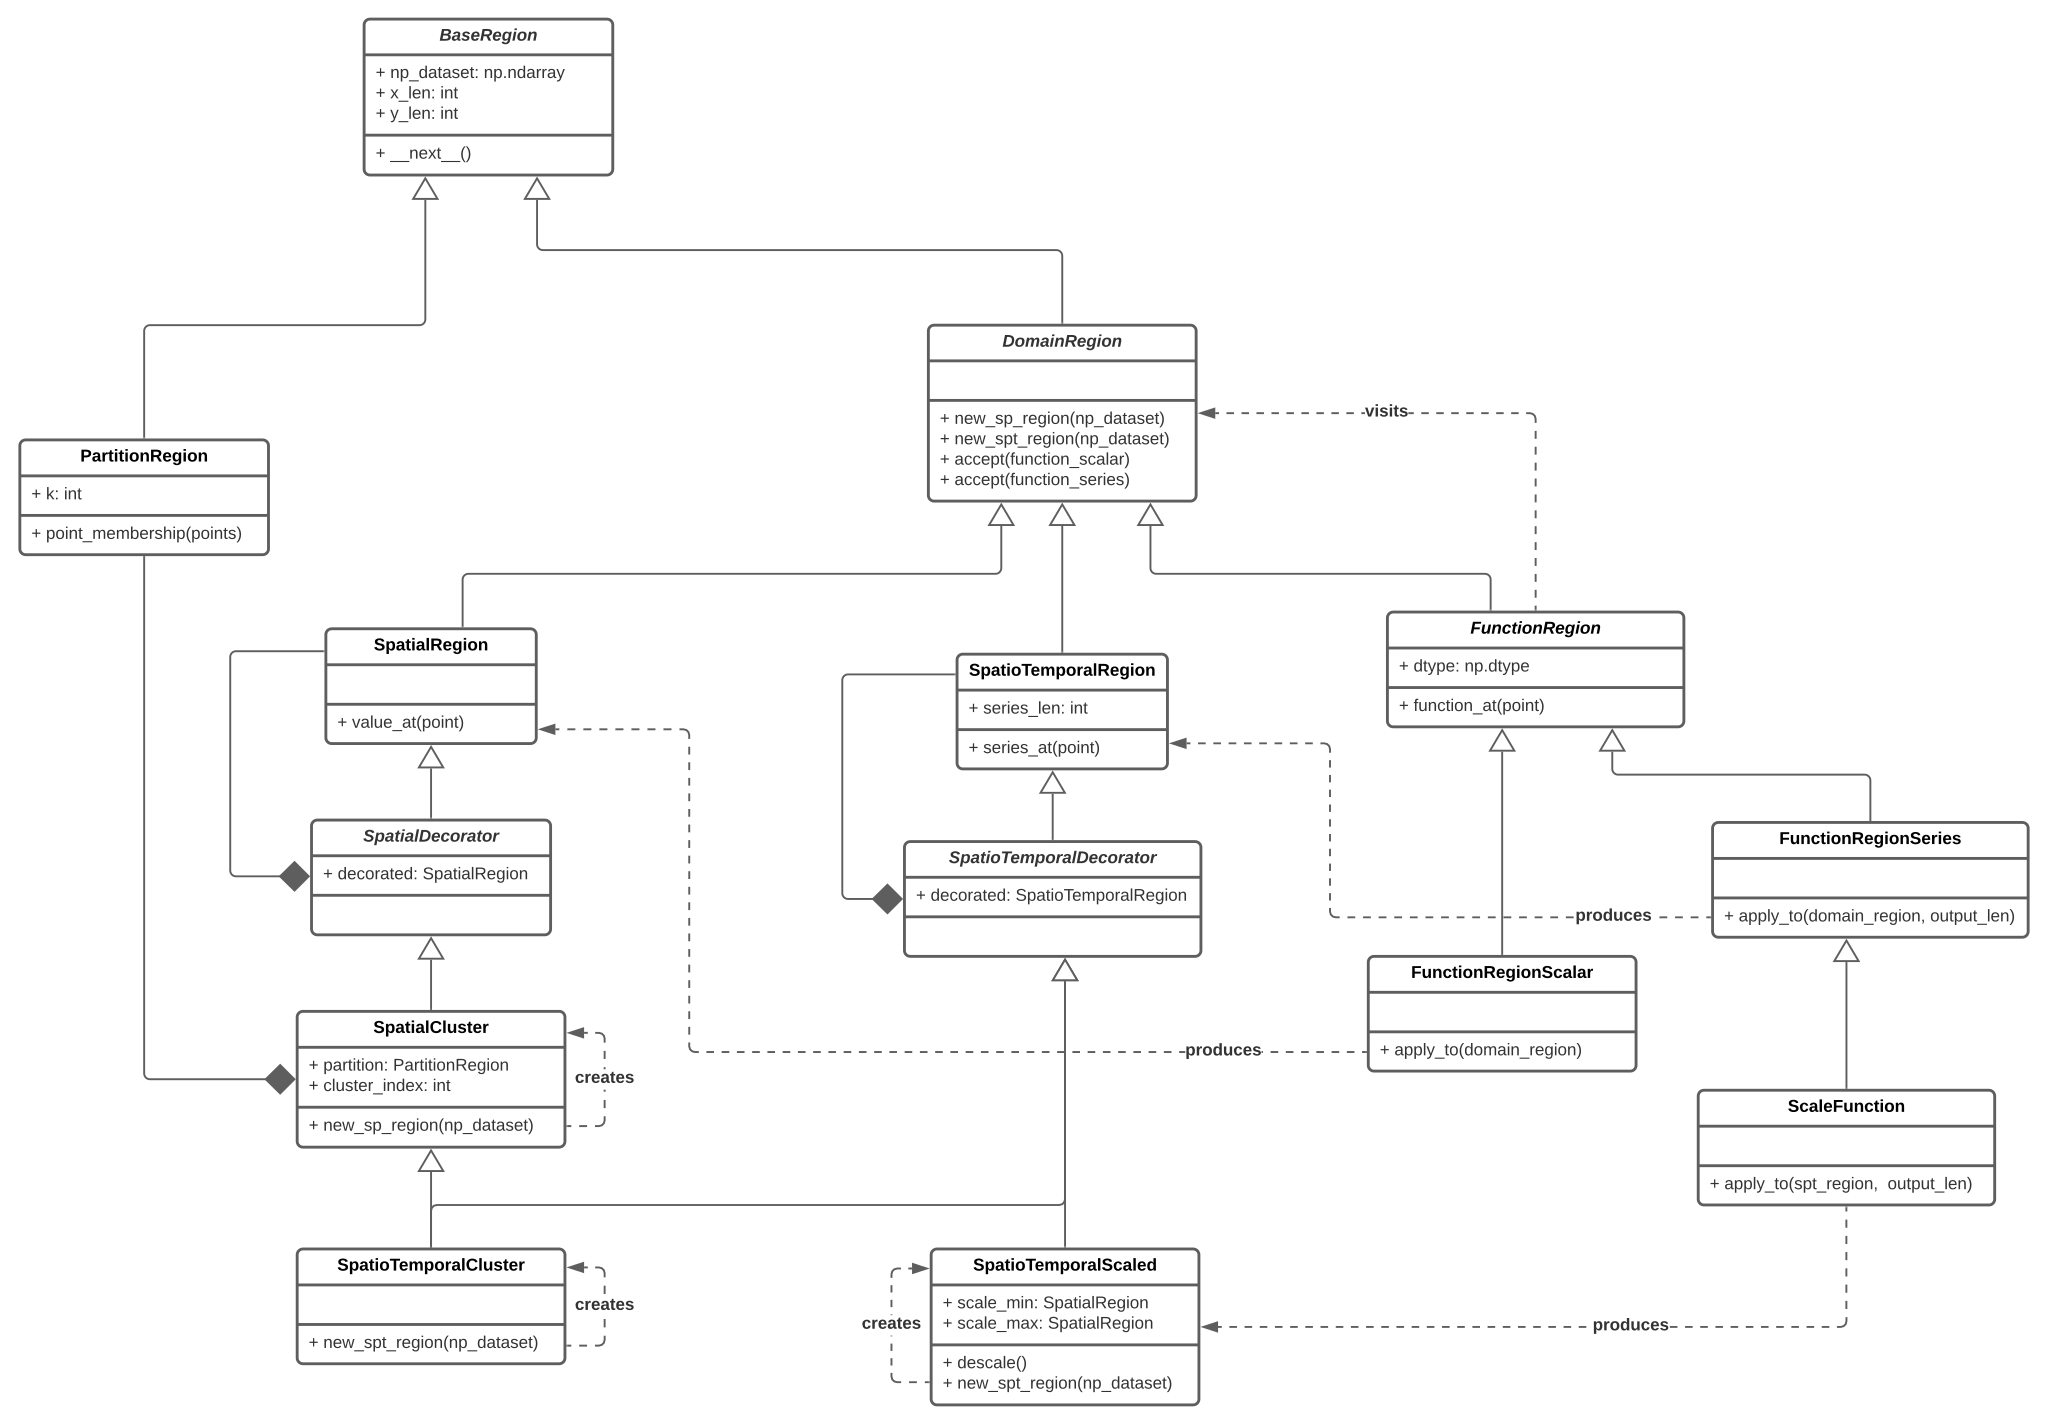
\includegraphics[scale=0.41, angle=90]{../Figures/SPT-TSA-RegionClasses}
	\caption{Class Diagram -Region Class.}	
	\label{Fig:DiagramClasess-Region}	 		
\end{figure}

%\Fab{Como teremos a Flavia na banca, ela vai olhar o Diagrama de Classes. Fui verificar a representação dos Decorators no livro "Design patterns" e me pareceu um pouco diferente. Tb. pareceu estranho Spatial Cluster e SpatioTemporal Cluster serevem especializações do Decorator. São eles tb. decoradores?}
% OK, a descricao dos Decorators foi esclarecida
A brief description of each class is provided:

\begin{itemize}
	\item \texttt{Point}: a simple implementation of a 2D position with $(x, y)$ coordinates.
	
	\item \texttt{BaseRegion}: The base class for all regions. It is a wrapper of a \texttt{numpy.ndarray} object, which constrains the dimensions of the region inside a 2D rectangle. In addition to providing basic functions such as saving a dataset to persistent storage, it allows the iteration of the domain points contained within the 2D boundary, using Point instances.
	
	\item \texttt{PartitionRegion}: Describes the application of a partitioning scheme to divide a spatio-temporal region into groups by storing the membership of each point in the region to a group. Note that it is kept separate from \texttt{DomainRegion} because it is not meant to accept function regions.
	
	\item \texttt{DomainRegion}: The parent class of both spatial and spatio-temporal regions and the operand and result of function regions. This abstract implementation has common functionalities for both 2D and 3D arrays, including interactions with function regions described below. Since function regions transform a domain region into a new region, we allow subclasses to determine which new instance to create by leveraging polymorphism. For example, a function region acting on an instance of \texttt{SpatialRegion} may produce a new \texttt{SpatialRegion} instance using the \texttt{new\_sp\_region} method declared in this class. However, that same function region acting on an instance of \texttt{SpatialCluster}, using the same \texttt{new\_sp\_region} method, will produce an instance of \texttt{SpatialCluster} instead, due to the polymorphic method call.
	
	\item \texttt{SpatialRegion}: The 2D implementation of \texttt{DomainRegion}, it stores a value at each point. Iterations of the points in the domain will yield the values for each point.
	
	\item \texttt{SpatioTemporalRegion}: The 3D implementation of \texttt{DomainRegion} stores an array at each point, representing a time series. Iterations on the points of a domain will yield the series for each point.
	
	\item \texttt{FunctionRegion}: A special type of \texttt{DomainRegion} used to transform \texttt{DomainRegion} instances, by accepting a \texttt{DomainRegion} instance as input and producing another \texttt{DomainRegion} instance as output, potentially of a different type. It serves as a common class for \texttt{FunctionRegionScalar} (produces a \texttt{SpatialRegion} instance as output) and \texttt{FunctionRegionSeries} (produces a \texttt{SpatioTemporalRegion} instance as output). The transformation of the input is achieved by storing a Python function at each point of the function region, and applying each function to the corresponding element in the operand region. To represent this application, consider a spatial region $S_{(m,n)}$ and a function region $F_{(m,n)}$, we then have $F(S) = \left\{ f_{ij}(s_{ij}); (i, j) \in [0, m]\times[0, n] \right\}$. Storing a function at each point is useful for some cases, e.g. when working with forecast models (each point can have its own model parameters). Additional subclasses are also available to store the same function in the entire region for computational efficiency. See \texttt{FunctionRegionScalar} for a practical example.
	
    The implementation uses the Visitor pattern, where the \texttt{DomainRegion} is the visitor that `visits' the function region to retrieve the corresponding function during an iteration of points. The benefit of the visitor approach is that the same \texttt{FunctionRegion} can be applied to different subclasses of \texttt{SpatialRegion} and \texttt{SpatioTemporalRegion} without knowledge of the particular subclasses while still producing different and expected outputs. A limitation of this approach is that only one function region can be applied to a given region at any given time. Otherwise, the iterator of the region will be used twice and become corrupted.
	
	\item \texttt{FunctionRegionScalar}: A subclass of \texttt{FunctionRegion} that produces a subclass of \texttt{SpatialRegion} when applied to a \texttt{DomainRegion}, regardless of the input domain being spatial or spatio-temporal. The implementation will call the \texttt{new\_sp\_region} method of the operand polymorphically to produce the desired output.
	
	For example, consider the problem of averaging each series in a spatio-temporal region by using the function \texttt{numpy.mean} to the series at each point of the region. It can be achieved by creating an instance of \texttt{FunctionRegionScalar} so that each point of its internal 2D array contains the function \texttt{numpy.mean} itself and applying this function region to the spatio-temporal region.
	
	\item \texttt{FunctionRegionSeries}: Analogous to \texttt{FunctionRegionScalar} but will always produce a subclass of \texttt{SpatioTemporalRegion} by calling the \texttt{new\_spt\_region} method of the input. It requires to know the length of the output series in advance in order to allocate the output 3D array.
	
	\item \texttt{ScaleFunction}: A subclass of \texttt{FunctionRegionSeries} that produces an instance of \texttt{SpatioTemporalScaled} (see below) when applied to a \texttt{SpatioTemporalRegion}.
	
	\item \texttt{SpatialDecorator}: The base decorator class in the implementation of the Decorator pattern for \texttt{SpatialRegion}. This pattern enables us to extend the functionality of a \texttt{SpatialRegion} by enclosing an instance of the region to perform additional operations. Also, decorators can be nested \cite{Gamma1994}. These properties are useful when creating subsets or transformations of a region, and we want the result to retain some of the original properties (e.g., clustered, with scaling).
	
	\item \texttt{SpatialCluster}: A decorator for \texttt{SpatialRegion} provides support for describing clusters obtained from a partitioning scheme. Each instance of \texttt{SpatialCluster} represents one group only (a group index is used), so $k$ instances would be required to represent the output of a partitioning scheme of $k$ groups. Iterations of \texttt{SpatialCluster} will only yield the points that are members of the corresponding group, and attempts to read the value of a point outside the group result in an error. This effect is achieved by keeping the same underlying data for all the $k$ instances (no additional copies are made) and the same instance of the  \texttt{PartitionRegion} but with a corresponding group index. The behavior is implemented by decorating the relevant methods in order to use the partition and the index.
	
	\item \texttt{SpatioTemporalDecorator}: The base decorator class in the implementation of the Decorator pattern, but this time for a \texttt{SpatioTemporalRegion}.
	
	\item \texttt{SpatioTemporalCluster}: A decorator for \texttt{SpatioTemporalRegion} that provides support for describing clusters obtained from a domain partitioning technique. This class uses multiple inheritances to also extend \texttt{SpatialCluster} in order to include cluster behavior, while at the same time working with a 3D array to store a series at each point.
	
	\item \texttt{SpatioTemporalScaled}: A decorator for \texttt{SpatioTemporalRegion} that represents the scaled version of a spatio-temporal region. The scaling process is performed by a \texttt{ScalingFunction}, which will iterate each point to scale the corresponding series independently. A series is scaled by finding its minimum and maximum values to generate the new values in the $[0, 1]$ interval. These minimum and maximum values are stored as two \texttt{SpatialRegion} instances inside the scaled region so that the original values can be restored at a later point. 
	
	Consider the example of partitioning a spatio-temporal region: this can be achieved b applying both the \texttt{SpatioTemporalCluster} and \texttt{SpatioTemporalScaled} decorators since it is possible to chain them. The expected output (a cluster representing a scaled series at each point) is obtained even if the decorators are applied in a different order. Reverting the scaling will yield a \texttt{SpatioTemporalCluster} again.
\end{itemize}

The second class diagram is shown in Figure \ref{Fig:DiagramClasess-Models}. The main focus is now the analysis of the forecast error. Here, we find classes related to the training of predictive models, their forecasting of future values of the predictive variable, and the subsequent calculation of the forecast error when the actual values are available. The descriptions provided here are for the relevant ARIMA predictive models. Other predictive models used as a baseline for comparison follow a similar class structure.

\begin{figure}[tp]
	%\begin{minipage}[b]{0.8\textwidth}
	\centering
	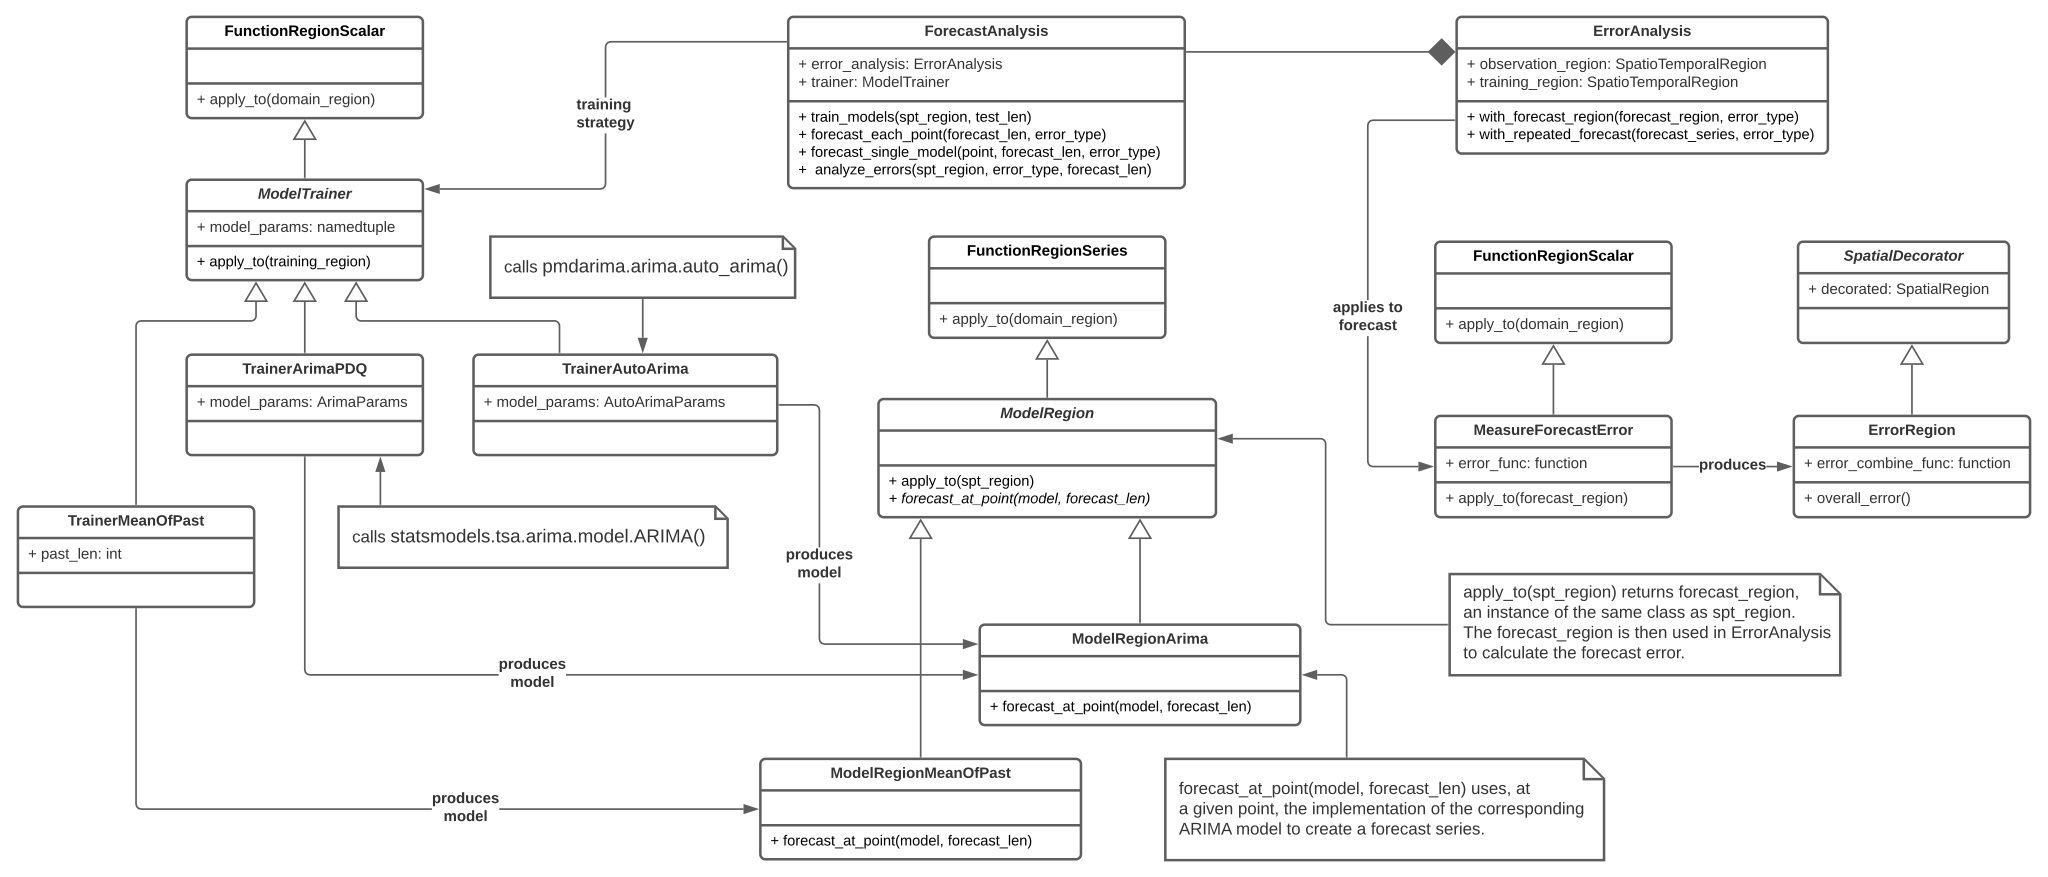
\includegraphics[scale=0.37, angle=90]{../Figures/SPT-TSA-ModelsClasses}
	\caption{Class Diagram -Model Class.}	
	\label{Fig:DiagramClasess-Models}	 		
\end{figure}

\begin{itemize}
	\item \texttt{ModelRegion}: Base class for the different predictive models supported by SPT-TSA. For each point in a spatio-temporal region, a model will produce a series that represents the predicted values of the predictive variable. It is achieved by extending the behavior of \texttt{FunctionRegionSeries}, where the length of the series represents the size of the forecast. If, for example, we pass an instance of \texttt{SpatioTemporalRegionScaled} as an operand, then the output is also scaled, and the original scaling information can be used to recover the desired forecast series.
	
	\item \texttt{ModelTrainer}: Base class for training predictive models supported by SPT-TSA. The models are trained by passing a training spatio-temporal region containing, for each point, a training series (same length for all points in the region). The implementation overrides the behavior of \texttt{FunctionRegionScalar} to produce an instance of \texttt{ModelRegion} instead of \texttt{SpatialRegion}. The exact class of the instance and its properties (resulting model parameters) will depend on the subclasses of \texttt{ModelTrainer} and how they process the \texttt{model\_params} input.
	
	\item \texttt{TrainerArimaPDQ}: A model trainer that will use, for each point, the class \\ \texttt{statsmodels.tsa.arima.model.ARIMA} to fit an ARIMA model using a training series and a $(p, d, q)$ tuple. The result of applying this function to a training region is an instance of \texttt{ModelRegionArima}.
	
	\item \texttt{TrainerAutoArima}: A model trainer that will use, for each point, \\
	\texttt{pmdarima.arima.auto\_arima} and a training series to determine the values for the $(p, d, q)$ tuple that maximize the AIC metric. The trainer will then use the training function of \texttt{TrainerArimaPDQ} to fit the resulting ARIMA model.
	
	\item \texttt{ModelRegionArima}: Represents the application of ARIMA as predictive model. It is a region that has an instance of \texttt{statsmodels.tsa.arima.model.ARIMAResults} at each point (the same instance could be referenced by many points if needed, this will save memory). When applied to a spatio-temporal region, it will create a new spatio-temporal region that holds, for each point, its corresponding forecast series given by \texttt{statsmodels.tsa.arima.model.ARIMAResults.forecast()}.
	
	\item \texttt{ErrorRegion}: A simple decoration of \texttt{SpatialRegion} that is meant to hold, for each point, a value representing the forecast error of some model. The decoration provides some additional functions for combining the errors in each point into a single metric, for example, using the RMSE.
	
	\item \texttt{MeasureForecastError}: Calculates the associated forecast errors between an observation region (an observed series in each point) and a forecast region (a forecast series). It leverages the implementation of \texttt{FunctionRegionScalar} to operate in each point with a given error metric, for example, RMSE. The result of applying this function region to a forecast region is an instance of \texttt{ErrorRegion}.
	
	\item \texttt{ErrorAnalysis}: A class that provides methods to calculate forecast errors using \texttt{MeasureForecastError} as a helper class. It can either apply the helper implementation directly given an entire forecast region or create a forecast region by repeating a single forecast series over each point of the observation region. This is useful when using the predictive model of a representative to create the same forecast for an entire region (\texttt{SpatioTemporalRegion}) or an entire group (\texttt{SpatioTemporalCluster}).
	
	\item \texttt{ForecastAnalysis}: Provides several strategies for training predictive models and evaluating their associated forecasts. It supports the training strategies described in the methodology, such as training a model at every point (naive approach) or training a model only at the representatives of each group. The second approach is designed so that each group is treated independently using \texttt{SpatioTemporalCluster} so that the actual implementation remains unaware of clusters: it uses the model of a single given point (meant to be the representative). It repeats it over the entire region using point iteration (will iterate only over the group members). This class also provides additional methods to calculate several associated errors, including the errors obtained when the forecast of every single model is repeated independently over the entire region. It allows the calculation of the `Model Composition with Minimal Local Error' and `Model Composition with Maximum Error' described in Section \ref{Sec:ModelRepresentatives}, they are found by exhausting every point in the region. Since the models can be analyzed independently, this calculation has been parallelized to improve efficiency.
\end{itemize}

\section{Final Considerations}
\label{Sec:implementation_summary}

In order to efficiently evaluate the methodology proposed in this work, the Spatio Temporal Tool for Time Series Analysis was designed and implemented. SPTA-TSA manages the tasks and operations considered in the offline and online phases of the methodology. It presents a simple command-line interface in scripts with the arguments needed to create domain partitionings, compute forecast errors and execute simple predictive queries. It was also used to perform the experimental results presented in the next chapter. Its object-oriented nature provided the necessary code organization to define experiments varying in several aspects, such as the domain partitioning technique, the predictive model, the error metric, and the model composition used.

For all of this, SPTA-TSA represents an important contribution to our work. While SPTA-TSA does not include a cost function for the spatio-temporal predictive query execution, this can be easily implemented, along with further extensions to turn the tool into a complete framework to explore predictive serving systems. \label{lastpage}